\documentclass{article}
\usepackage{proj1}
\usepackage{natbib}
\usepackage{amsmath}
%set spacing between lines (DO NOT CHANGE SPACING)
\linespread{1.25} %normally 1.25
\setlength{\parindent}{0cm}
\graphicspath{{Images/}}
%\underline{\smash{\beta}} makes underlining at the same distance

%Definition of margins (DO NOT ALTER!)+

%\usepackage[a4paper, top=1in, left=1.0in, right=1.0in, bottom=1in, includehead, includefoot]{geometry} %Usually have top as 1in

%%%%%%%%%%%%%%%%%%%%%%%%%%%%%%%%%%%%%%%%%
% +++ ... +++ denotes something to be changed
%%%%%%%%%%%%%%%%%%%%%%%%%%%%%%%%%%%%%%%%%%
%Commands
\newcommand{\PDEsmall}[2]{\frac{\partial #1}{\partial #2}}
\newcommand{\PDE}[2]{\dfrac{\partial #1}{\partial #2}}
\newcommand{\folds}{(x_0,y_0)}
\newcommand{\st}{such that }
\newcommand{\wrt}{with respect to }
\newcommand{\vdp}{Van der Pol }
%%%%%%%%%%%%%%%%%%%%
\title{Fast Slow Dynamics - the van der Pol Oscillator}
\author{}
\date{October 2018}

\begin{document}

\maketitle

\section{Setup}
We wish to study the behaviour of the van der Pol oscillator using blow up. The van der Pol oscillator is a well-studied second order ODE used to model a variety of physical and biological phenomena. A position coordinate \(x(t)\) evolves according to the following equation. 
\begin{equation} \label{eq:vdP}\ddot{x}(t)-\mu\left(1-x^2(t)\right)\dot{x}(t)+x(t)=0   \end{equation}
Here, \(\mu \gg 1\) is a scalar constant. \par 

Currently, it doesn't resemble a anything like what we've seen in \cite{krupa2001}. To make it resemble a fast/slow system, we introduce a new variable. Let \(w=\dot{x}+\mu F(x)\) where \(F(x)=\frac{x^3}{3}-x\). Why have we chosen this function \(F\)? Notice that \(F'(x)=-(1-x^2)\), our nonlinear term in Equation \ref{eq:vdP}. Differentiating \(w\) we obtain
\begin{align*}
    \dot{w}&=\ddot{x}+\mu\od{}{x}\left(\frac{x^3}{3}-x\right)\od{x}{t}\\
    & =\ddot{x}+\mu(x^2-1)\dot{x}\\
    &= -x
\end{align*}
Here, the last equality follows from the van der Pol equation. We now have a two dimensional system.
\[\begin{cases} \dot{x}=w-\mu F(x)\\
 \dot{w}=-x\end{cases}\]
 Let \(y=\frac{w}{\mu}\). Then
 \[\begin{cases} \dot{x}=\mu\left(y-F(x)\right)\\
 \dot{y}=-\frac{x}{\mu}\end{cases}\]
We will pause here although it doesn't look quite right and do a phase plane analysis to better understand the behaviour of the system. Setting each equation equal to zero in turn gives nullclines of \(x=0\) and \(y=F(x)\). 

+++ PHASE PLANE ANALYSIS +++

+++ New transformation to fast/slow system +++


Fast System:
\begin{equation}\label{fastsystem}
    \begin{cases} x'=y-F(x)\\
    y'=-\epsilon x
    \end{cases}
\end{equation}


Slow system:
\begin{equation}\label{slowsystem}
    \begin{cases} \epsilon \dot{x}=y-F(x)\\
    \dot{y}=-x
    \end{cases}
\end{equation}

\subsection{Fold Points}\label{Fold Points}
The fold points are $(x_0^+,y_0^+)=(1,-\dfrac{2}{3})$ and $(x_0^-,y_0^-)=(-1,\dfrac{2}{3})$
\begin{figure}[h]
    \centering
    %\includegraphics{}
    \caption{Our Manifold $f(x,y,\epsilon)$}
    \label{fig:my_label}
\end{figure}

\subsection{Non-degeneracy}
Now that we have established our fast-slow systems (Equation \ref{fastsystem} and \ref{slowsystem}) we need to check our non-degeneration conditions \citep{krupa2001}. 
%Before proceeding it is prudent to note that the nondegeneracy conditions will be opposite for the case where $(x_0,y_0)=(x_0^+,y_0^+)$ to satisfy our system.
Now we first check that $ \pd{^2f}{x^2}(x_0,y_0,0)\neq 0$ then we have,
\begin{equation}
    \pd{^2}{x^2}(y-\dfrac{x^3}{3}-x)=-2x,
\end{equation}
which we can evaluate at our fold points (Section \ref{Fold Points}) to give,
\begin{equation} 
    \begin{cases}
            &\pd[2]{f}{x}(x_0^+,y_0^+,0)=2<0\\
            &\pd[2]{f}{x}(x_0^-,y_0^-,0)=2>0.
    \end{cases}
\end{equation}
Then we can consider that $\pd{f}{y}(x_0,y_0)\neq 0$. We show this by the following,
\begin{align}
        &\pd{f}{y}(x_0^+,y_0^+,0)=1\\
        &\pd{f}{y}(x_0^-,y_0^-,0)=1.
\end{align}
Lastly we need to consider that $g(x_0,y_0,0)\neq 0$. This is easily seen as we find that $g(x_0,y_0,0)=\pm 1$ for our two fold points. From here we are can now consider our transformation.

\section{Charts}\label{sec: charts}
include picture from the book \begin{figure}[h!]
    \centering
    %\includegraphics{}
    \caption{Charts}
    \label{fig: charts}
\end{figure}
\section{Transformation}
\citet{krupa2001} discusses why we should make a transformation for our system. We find that if we map $\folds=(0,0)$ we are then able to simplify our non-degeneracy conditions - as shown in Equation \ref{non-degeneracy} \citep{krupa2001}.
\begin{equation}
    \begin{cases}
        &\folds=(0,0)\\
        &\pd{^2f}{x^2}(0,0,0)>0\\
        &\pd{f}{y}(0,0,0)<0
    \end{cases} 
    \label{non-degeneracy}
\end{equation}

\subsection{Mapping Transformation}\label{sex: mapping}
To be able to continue with our analysis we should consider the transformations. We will first only consider the case for our fold point at $(x_0^+,y_0^+)=(1,-\dfrac{2}{3})$. We wish to map $(x,y)\to (1-\Tilde{x},\Tilde{y}-\frac{2}{3})$ which reflects and translates our system \st our fold points are now mapped to $(0,0)$ - Figure \ref{fig: Transformed System}. 

\begin{figure}[h]
    \centering
    %\includegraphics{}
    \caption{Our transformed system.}
    \label{fig: Transformed System}
\end{figure}
Now that we have made our transformation we can check our non-degeneracy conditions. However, before we continue we should check that our the sign of the derivative is conserved through the transformation. We can do this by using the chain rule as follows, 

\begin{equation}
    \od{x}{t}=\od{\Tilde{x}}{x}\od{x}{t}=-\od{\Tilde{x}}{t}. \label{chain rule}
\end{equation}
Now using Equation \ref{chain rule} and our new mapping ( $(x,y)\to (1-\Tilde{x},\Tilde{y}-\frac{2}{3})$) we are able to define our new Fast System in the following way, 
\begin{equation}
    \begin{cases}
        x'=-y+x^2-\dfrac{(x)^3}{3}\\
        y'=\epsilon(x-1)
    \end{cases}
    \label{eq: Fast System}
\end{equation}
where we note that we have dropped the tilde on $x \ \text{and} \ y$ for convenience. \\

\subsection{Non-degeneracy Conditions}
\begin{equation}
    \begin{cases}
        &\folds=(0,0)\\
        &\pd[2]{f}{x}(0,0,0)>0\\
        &\pd{f}{y}(0,0,0)<0
    \end{cases} 
    \tag{\ref{non-degeneracy}}
\end{equation}
Now that we have constructed our transformed system, we are now able to check our non-degeneracy conditions - Equation \ref{non-degeneracy}. It is clear to see that $\folds=(0,0)$ by the mapping we defined in Section \ref{sex: mapping}. Following this we are able to check our other non-degeneracy conditions conform to our new mapping. The differentiation is easily seen from Equation \ref{eq: Fast System} which yields that $\pd[2]{f}{x}(0,0,0)=2>0$ and $\pd[1]{f}{y}(0,0,0)=-1<0$, confirming our assumptions.


\subsection{Reduced Dynamics}
The next progression for our system is to consider the reduced dynamics within our system. To do this we consider Equation \ref{slowsystem} and take the $\epsilon\to0$ which yields the following system,
\begin{subequations}
    \begin{align}
    &0=f(x,y,0)=-y+x^2-\dfrac{x^3}{3}\\
        &\dot{y}=g(x,y,0)=0 \label{eq: reduced g}
    \end{align}
\end{subequations}
which is known as the slow subsystem \citep{Bible}. We are then able to compute the reduced flow by computing  \citep{krupa2001},
\begin{equation}
    \phi_x(x)\dot{x}=g(x,\phi(x),0),\text{ for }y=\phi(x).
    \label{eq: general reduced}
\end{equation}
We find that $\phi(x)=x^2-\dfrac{x^3}{3}$ where the derivative \wrt $x$ gives $\phi_x(x)=2x-x^2$. Now it is clear that we will have a singularity at $x=0$, by Equation \ref{eq: general reduced}, thus we will find that our system blows up ($\dot{x}\to\infty$) which motivates the process that will follow. \\ \\
%note that the sign g(0,0,0) determines the flow direction 
%g(0,0,0)<0 as expected in our example.
After finding our reduced system we are able to determine the way in which it flows by considering the sign of $g(0,0,0)$. We see from Equation \ref{eq: reduced g} that $g<0$ then we have that our flow is directed towards the fold points $(0,0)$. To continue with our analysis we first need to define Fenichel's theorems.

\subsection{Fenichel and Standard Theory}
\textbf{THEOREM}

\subsection{Extended System}
Now that we have established the above theorems then we need to consider the extended system \st $\epsilon'=0$, thus $\epsilon=\text{\textit{const}}$. By considering this system we will be able to consider a blow up (magnification) around our fold point in three dimensions.  
\begin{figure}[h]
    \centering
%    \includegraphics{}
    \caption{Blown up system}
    \label{fig: blow up}
\end{figure}
From Figure \ref{fig: blow up} we can consider the stability of our fold point. To do this we are able to establish the following determinant,
\begin{equation} 
    A=\begin{vmatrix} 2x-x^2-\lambda & -1&0 \\ 0 & -\lambda&0\\0&0&-\lambda \end{vmatrix}=\lambda^2(2x-x^2-\lambda).
    \label{eq: Eigenvalues}
\end{equation}
However, a far easier approach is to note that our matrix is an upper triangular matrix which we can take the eigenvalues directly from Equation \ref{eq: Eigenvalues} \st $(\lambda_1.\lambda_2,\lambda_3)=tr(A)$. Then we can clearly see that for our fold points $\lambda_i=0 \ \text{for} \ i=1,2,3$ and for any $x\neq0$ we have $\lambda_1=x(2-x)$ and $\lambda_2=\lambda_3\equiv0$. As a result we can see that we are forced to blow up our system around our fold point as our steady states are non-hyperbolic whereas outside of this we find that we have one hyperbolic steady state.
%Now we can see that we have three non-hyperbolic eigen values when we consider our system at (0,0,0), 


\subsubsection{Canonical Form}
Now that we have established our reduced system we are able to rewrite it in canonical form - Equation \ref{eq: canonical}.
\begin{equation}
    \begin{aligned}
        &x'=-y+x^2-\frac{x^3}{3}=-y+x^2+h(x) \\
        &y'=\epsilon(x-1)
    \end{aligned}
    \label{eq: canonical}
\end{equation}
There is ample reasoning for doing this. This is because we find that the canonical form has been studied in great detail allowing us to make comparisons and to avoid excess computation. This then allows us to follow an analogous approach to the many papers associated with this topic - as seen in \citet{krupa2001} paper on Extending Geometric Singular Perturbation Theory.

\section{Blow-ups in our System}\label{sec: VDP Blowup}
We first need to transform our system in a new coordinate and time system. This is because we are considering our point as a circle with radius zero. By doing this we are then able to consider a localised flow within our system which is a most on the boundary of our point ($r=0$). To do this we need to consider varying powers of $r$ in each of our variables \st we have the system shown in Equation \ref{sys: blow up trans}.  
\begin{subequations}
    \begin{align}
        &x=\Bar{r}\Bar{x}  \label{sys: blow up trans x}\\
        &y=\Bar{r}^2\Bar{y} \label{sys: blow up trans y}\\ 
        &\epsilon=\bar{r}^3\bar{\epsilon} \label{sys: blow up trans z}
    \end{align}  
    \label{sys: blow up trans}
\end{subequations}
Now that we have this transformation we are then able to consider our charts (see Section \ref{sec: charts}) in our system.

\subsection{Charts}
We note that our system will have three charts $ K_1,K_2,K_3 $, where we have $ \bar{y}=1, \ \bar{\epsilon}=1, \ \bar{x}=1 $. By inserting these into Equations \ref{sys: blow up trans x}, \ref{sys: blow up trans y} and \ref{sys: blow up trans z} respectively to give, 
\begin{subequations}
	\begin{align}
	&x=r_1x_1, \ y=r_1^2, \ \epsilon=r_1^3\epsilon_1,\\
	&x=r_2x_2, \ y=r_2^2y_2, \ \epsilon=r_2^3 \label{sys: K2}\\
	&x=r_3, \ y=r_3^2y_3, \ \epsilon=r_3^3\epsilon_3\label{sys:K3}
	\end{align}
\end{subequations}
where $ (x_i,r_i,\epsilon_i)\in\Re^3 $ for $ i=1,2,3 $ \citep{krupa2001}. Now that we have done this we can consider the individual charts explicitly. We start with chart two ($K_2$) for a simple reason. This is because we area able to glean the most information out of this chart. We will see that we then find that we can define the mappings from chart one to two and two to three, further simplifying our analysis in the future.

\subsection{Dynamics in \texorpdfstring{$K_2$}{K2}} \label{sec: VDP K_2}
To be able to consider chart $ K_2 $ %Ask Nikola why he starts with K_2
we will use the transformation - shown in Equation \ref{sys: K2} - in our canonical system. We also need to use a time rescaling ($ t_2=r_2t $) to be able to desingularise the system. Now substituting this into Equation \ref{eq: canonical} yields,
\begin{align}
&\od{}{t}(r_2x_2)=r_2^2\od{x_2}{t}=-y_2+x_2^2-\dfrac{x_2^3r_2}{3},\\
&r^3_2y'_2=r^3_2(-1+r_2x),\\
&r'_2=0,
\end{align}
noting that $ \od{r}{t_2}=\od{t}{t_2}\od{r}{t}=\frac{1}{r_2}\od{r_2}{t} $ and we are taking the equations to $ O(r_2) $. Now dividing through by $ r^2_2 $ and $ r^3_2 $ respectively for each equation we get,

\begin{equation}
	\begin{aligned}
		&x'_2=x^2_2-y_2+O(r_2),\\
		&y'_2=-1+O(r_2),\\
		&r'_2=0,
	\end{aligned}
\end{equation}
which are then able to evaluate as a layer problem. Now we know that this is the Riccati Equation - see \citet{Riccati}.
%+++++ Riccati equations not the ones above but the ones that satisfy r_2=0++++++++++++++++++++++

\subsection{Dynamics in \texorpdfstring{$K_1$}{K1}}

\subsection{Dynamics in \texorpdfstring{$K_3$}{K3}}
Similarly to $K_1$ and $K_2$, the system can be transformed using Equation \ref{sys:K3}.
\begin{align*}
\od{r_3}{t_3}&=r_3F(r_3,y_3,\epsilon_3)\\
\od{y_3}{t_3}&=\epsilon_3(r_3-1)-2y_3F(r_3,y_3,\epsilon_3)\\
\od{\epsilon_3}{t_3}&=-3\epsilon_3F(r_3,y_3,\epsilon_3)
\end{align*}
where $F(r_3,y_3,\epsilon_3)=\left(1-y_3-\frac{r_3}{3}\right)$
\newpage
\section{Canard Points}
During this section we will be considering a canard point. This is when our fold point is shifted along the manifold - Figure \ref{fig: Canard Point}. 
\begin{figure}[h!]
    \centering
    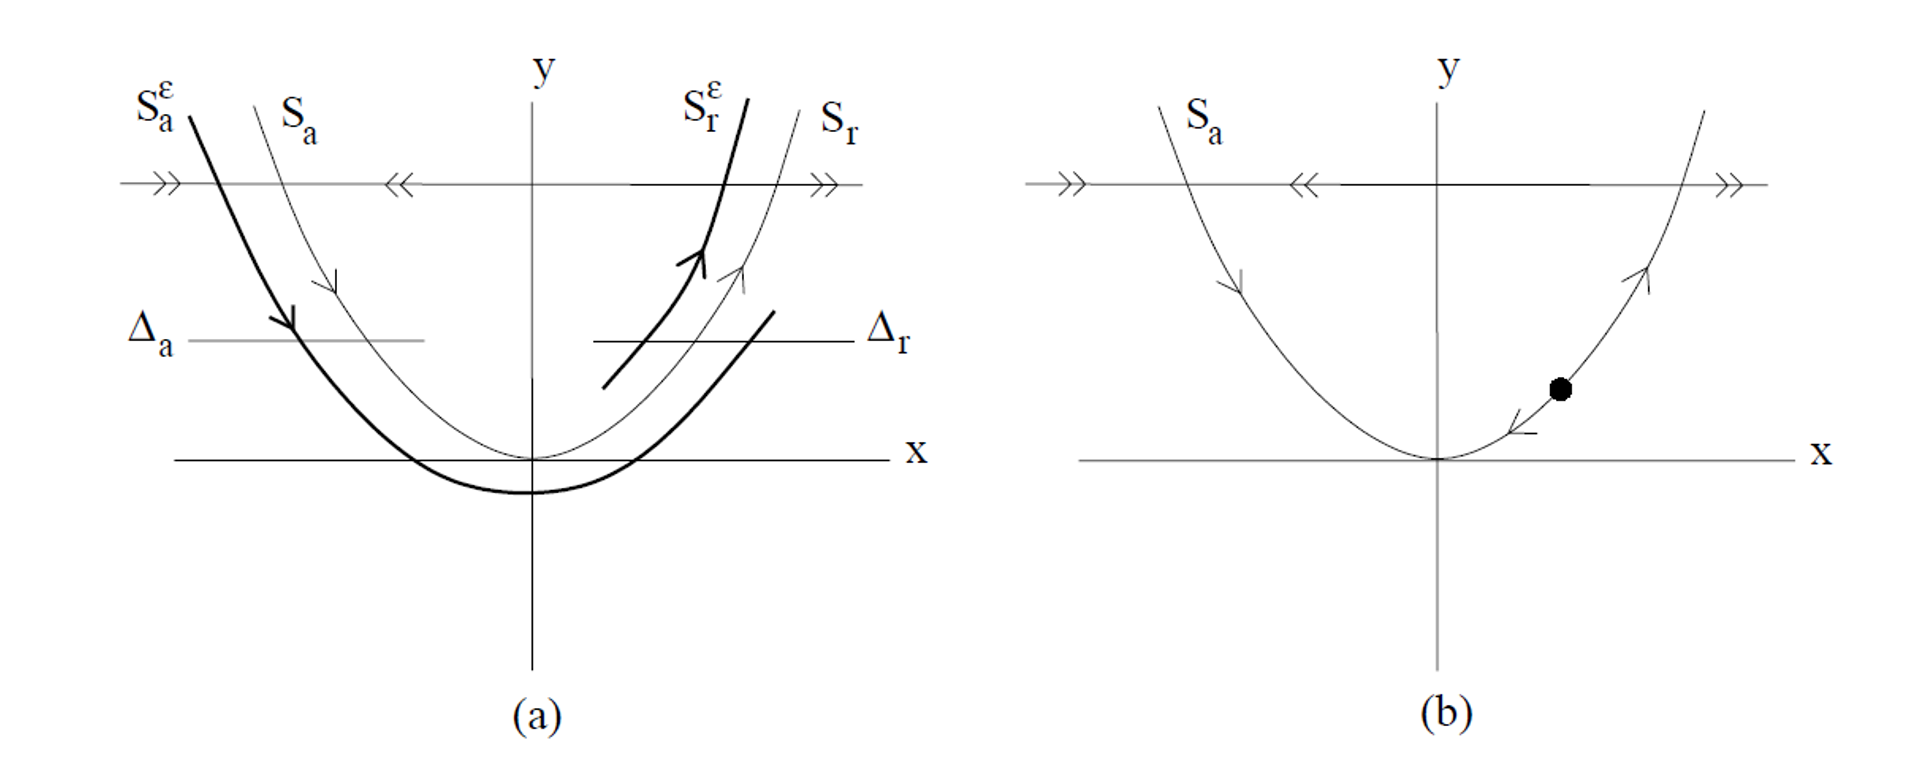
\includegraphics[height=5cm,width=8cm]{Canard_Point.png}
    \caption{The reduced flow of our system for a) $\lambda=0$ and b) $\lambda>0$.}
    \label{fig: Canard Point}
\end{figure}
To adequately explain the effect that the canard point will have on our system we will need to consider our system,
\begin{equation}
     \begin{aligned}
        &x'=-y+x^2-\dfrac{x^3}{3},\\
        &y'=\epsilon(x-1),\\
        &\epsilon'=0.\\
        % &\lambda'=0,\\
     \end{aligned}
    \tag{\ref{eq: Fast System}}
\end{equation}
Now we need to consider Equation \ref{eq: Fast System} in terms our our cananrd system. To do this we rewrite our system with an extra parameter $\lambda$, where $\lambda$ is our perturbation of our fold point \citep{krupa2001}. \citet{krupa2001} discusses generally how we should continue with computing our canard system. If we apply his theory to the \vdp system we find,
\begin{equation}
     \begin{aligned}
        &x'=-y+x^2-\dfrac{x^3}{3},\\
        &y'=\epsilon(x-\lambda),\\
        &\epsilon'=0,\\
         &\lambda'=0,\\
     \end{aligned}
        \label{eq: canard system}
\end{equation}
where the change in $\epsilon$ and $\lambda$ are constant. Now, for the remainder of the section, we follow the method of \citet{krupa2001} for the canard system. If we start by rewriting our canard system into the canonical forms we find,
\begin{align}
      &x'=-yh_1(x,y,\epsilon,\lambda)+x^2h_2(x,y,\epsilon,\lambda),\\
        &y'=\epsilon(xh_4(x,y,\epsilon,\lambda)-\lambda h_6(x,y,\epsilon,\lambda)),\\
\end{align}
Where we note that $h_j(x,y,\epsilon,\lambda)=1+O(x,y,\epsilon,\lambda)$ for $j=1,2,4,5$ and $h_3(x,y,\epsilon,\lambda)=O(x,y,\epsilon,\lambda)$. However, we should note that for the \vdp system our only term that is not solely of leading order is $h_2(x,y,\epsilon,\lambda)=1-\frac{x}{3}$. Now we are able to choose such a $\lambda>0$ that produces an equilibrium on our repelling branch $S_r$ for the reduced flow. By doing this we are then able to define the following conditions for our reduced flow on $h_j$,
\begin{align}
    &a_3=\pd{}{x}h_2(0,0,0,0)=-\frac{1}{3},\\
    &A=-a_2+3a_3-(2a_4+2a_5)=-1,
\end{align}
where we notice that our other solutions for $a_i=0$ for $i=1,2,4,5$ are trivial. The reason that we consider the constant $A$ is because we will find that this constant is crucial in our canard point analysis iff $A\neq 0$ \citep{krupa2001}. Following this \citep{krupa2001} discusses the existence of a critical value for $\lambda$ (denoted $\lambda_c$), where our two branches $S_r$ and $S_a$ must connect in a smooth fashion. Now from \textit{Theorem 3.1} we nkow that we must have a transition map at our critical point,
\begin{equation}
    \lambda_c(\sqrt{\epsilon})=-\epsilon(\frac{a_1+a_5}{2}+\frac{A}{8})+O(\epsilon^\frac{3}{2}),
\end{equation}
which can be written as $\lambda_c(\sqrt{\epsilon})=\frac{\epsilon}{8}+O(\epsilon^\frac{3}{2})$ for the \vdp system \citep{krupa2001}. Consider Canard cycles and center manifolds / Freddy Dumortier, Robert Roussarie. for more details on canards in \vdp.


\subsection{Canard Blow-up}
Now similarly to Section \ref{sec: VDP Blowup} we consider various transformations of our coordinate system to be able to be able to consider the non-hyperbolic equilibrium induced by our canard point. However, as we would expect with our new system we should consider a new set of transformations \citep{krupa2001}.
\begin{equation}
    x=\bar{r}\bar{x}, \ y=\bar{r}^2y, \ \epsilon=\bar{r}^2\bar{\epsilon}, \ \lambda=\bar{r}\bar{\lambda}
\end{equation}
Now that we have established the transformation we can then define our transformations for $K_1$ and $K_2$ but it is not necessary to consider the third chart ($K_3$). This is because we find that the attracting slow manifold connects to the repelling slow manifold. As a result of this we find that our flow will `bend back' from $K_2$ into $K_1$ instead of flowing out into the fast flow, which is described by $K_3$. This concept can be described by the Figure \ref{fig: flow in canard}.
\begin{figure}[h!]
    \centering
    \includegraphics{}
    \caption{Figure describing canard flow in manifold}
    \label{fig: flow in canard}
\end{figure}

\\
Since we have established why we need only consider two charts we can our transformations,
\begin{subequations}
    \begin{align}
        &x=r_1x_1, \ y=r_1^2, \ \epsilon=r_1^2\epsilon_1, \ \lambda=r_1\lambda_1 \label{eq: coordiante K_1}\\ 
        &x=r_2x_2, \ y=r_2^2y_2, \ \epsilon=r^2_2, \ \lambda=r_2\lambda_2 \label{eq: coordinate K_2}
    \end{align}
\end{subequations}
Since these transformations have been defined we should consider our charts. We will first consider chart 2, for analogous reasoning to Section \ref{sec: VDP K_2}. 

\subsubsection{Dynamics in $K_2$}
We start by noting that we are considering our invariant plane at $r_2=0$ which will significantly simplify our system for $K_2$. Further we should note that we are taking a transformation in time, $\od{r}{t_2}=\od{t}{t_2}\od{r}{t}=\frac{1}{r_2}\od{r_2}{t}$, as well as in our coordinates. Then if we substitute our time transformation and Equation  \ref{eq: coordinate K_2} into our system of Equations \ref{eq: canard system} we find, 
\begin{subequations}
    \begin{align}
    r_2^2x_2' - r_2x_2r_2'&=-r_2^2y_2h_1+r^2_2x^2_2h_2,\notag\\
    \implies x_2&=-y_2+x_2^2-r_2G_2(x_2,y_2),\\
%     \end{aligned}
% \end{equation*}
% \begin{equation}
%     \begin{aligned}
        r^3_2y_2'-3r_2^2y_2r_2'&=r^2_2(r_2x_2h_4-r_2\lambda_2h_5),\notag\\
        \implies y_2'&=x_2-\lambda_2+r_2G_2(x_2,y_2), \label{eq: K_2 y trans}
    \end{align}
\end{subequations}
where we note that $h_j=h_j(x,y,\epsilon,\lambda)$ for $j=1,2,3,4,5$. We should also recall that $r_2'=\lambda_2'=0$. Notice that we have included an additional term in Equation \ref{eq: K_2 y trans} - we define $G_2(x_2,y_2)$ in the following way, $G(x_2,y_2)=(G_1(x_1,y_1),G_2(x_2,y_2))^T=(-\frac{x^2_2}{3},0)^T$. The reason we also define this vector is to aide in the Melnikov computations which we will see later. \citet{krupa2001} discusses that for this chart we have an interesting result. They note that at $r_2=\lambda_2=0$ our system is integrable which allows us to define a constant of motion $H(x_2,y_2)=\frac{1}{2}\exp{(-2y_2)}\left(y_2-x^2_2+\frac{1}{2}\right)$ which we can easily verify \citep{krupa2001} using the following equations,
\begin{align*}
    x'_2&=e^{2y_2}\pd{H}{y_2}(x_2,y_2),\\
    y_2'&=-e^{2y_2}\pd{H}{x_2}(x_2,y_2).
\end{align*}
\textbf{Further to this we can see, when we consider our reduced system, that we have an equilibrium at the origin, implying that $H(x_2,y_2)=h$. This then allows us to define a trajectory for the orbit by\\
WHY??????????}
\begin{equation}
    \gamma_{c,2}(t_2)=(x_{c,2}(t_2),y_{c,2}(t_2))=\left(\frac{t_2}{2},\frac{t^2_2}{4}-\frac{1}{2}\right)    
\end{equation}
Next we will be continuing our analysis onto $K_1$.


\subsection{Dynamics in $K_1$}
For $K_1$ we follow a similar approach to the above. We will use the transformations, 
\begin{equation}
         x=r_1x_1, \ y=r_1^2, \ \epsilon=r_1^2\epsilon_1, \ \lambda=r_1\lambda_1 \tag{\ref{eq: coordiante K_1}},
\end{equation}
to find the relevant pathways of our flows. Now if we first consider the $r_1$ component, 
\begin{align}
    2r_1^2r_1'=r_1^2\epsilon(r_1x_1-r_1\lambda_1), \label{canard: r_1}
\end{align}
where we can call $F=F(x,y,\epsilon,\lambda)=x_1-\lambda_1+O(r_1(r_1+\lambda_1)$. Now we will see the motivation with starting with $y=r_1$ when we transform our other coordinates. Now if we consider $x=r_1x_1$,
\begin{align*}
    r_1r_1'x_1+r_1^2x_1'&=-r_1^2+r_1^2x_1^2,\\
    x_1'&=-1+x_1^2-\frac{x_1r_1'}{r_1},
\end{align*}
where we can use Equation \ref{canard: r_1} to simplify this further - Equation \ref{eq: canard x_1}.
\begin{align}
    x_1'=-1+x_1^2-\frac{x_1}{r_1}\left(\frac{r_1\epsilon_1F}{2}\right) \label{eq: canard x_1}
\end{align}
We now consider our $\epsilon=\epsilon_1r_1^2$ and noting $\epsilon'=0$. Then we have, $r_1^3\epsilon'=-2r_1^2\epsilon_1r_1'$, where we can use Equation \ref{canard: r_1} to simplify to,
\begin{align}
    \epsilon'=-\epsilon_1^2F. \label{canard: epsilon k_1}
\end{align}
Our last transformation is for our new coordinate $\lambda=r_1\lambda$, noting that $\lambda'=0$. Similarly to the above we find $r_1^2\lambda_1'+r_1\lambda_1r_1'=0$ then, 
\begin{equation}
    \lambda'_1=-\frac{\lamda_1\epsilon_1F}{2}, 
\end{equation}
which is a trivial rearrangement as seen in Equation \ref{canard: epsilon k_1}. Now if we combine the above we find that our transformed system is of the following form,
\begin{subequations}
    \begin{align}
            r_1'&=\frac{\epsilon}{2}(r_1x_1-r_1\lambda_1), \\
            % \label{canard: r_1}
            x_1'&=-1+x_1^2-\frac{x_1\epsilon_1F}{2},\\
            \epsilon'&=-\epsilon_1^2F,\\
            \lambda'_1&=-\frac{\lamda_1\epsilon_1F}{2}.
    \end{align}
    \label{canard: system of equations}
\end{subequations}
% Unique becuase of exponetial attraction in canard case - note it is the reversal of figure 2.4 for uniqueness
From this system we are now able to make some deductions. We first can observe that the hyperplanes are along the $r_1=\epsilon_1=\lambda_1=0$ with an invariant line at $l_1=\{(x_1,0,0,0): x_1\in\Re\}$ \citep{krupa2001}. As \citet{krupa2001} discusses the equilibria present at the end of both of our branches - Figure \ref{fig: Canard Point} - which are found at $p_a=(-1,0,0,0) \ \text{and} \ p_r=(1,0,0,0)$ \citep{krupa2001}. Now we can go one step further, we can consider Equation \ref{canard: system of equations} and find the eigenvalues of the system for the invariant planes. We find that, 
\begin{equation}
    J-\lambda I= \begin{bmatrix}
    2x-\lambda & 0 & 0 & 0  \\
    0 & -\lambda & 0 & 0&\\
    0 & 0 & -\lambda & 0 \\
    0 & 0 & 0 & -\lambda
\end{bmatrix},
\end{equation}
which clearly has three zero eigenvalues and one non-zero eigenvalue $\lambda=\pm 2$. Which further empahsises that our equilibrium point is non-hyperbolic.  
% \begin{align}
%     \label{canard: x_1}
% \end{align}







% This effect can cause numerous effects within applications of dynamical systems. 



\newpage
\appendix
\section{Dynamics in \texorpdfstring{$K_2$}{K2}}

\newpage
\bibliography{FastSlow.bib}
\bibliographystyle{agsm}
\nocite{strogatz2007nonlinear}
\appendix
\section{Log}
\end{document}
